\section{Model}
\label{sec:model}

\begin{figure}
  \begin{centering}
    \begin{subfigure}[b]{0.58\textwidth}
      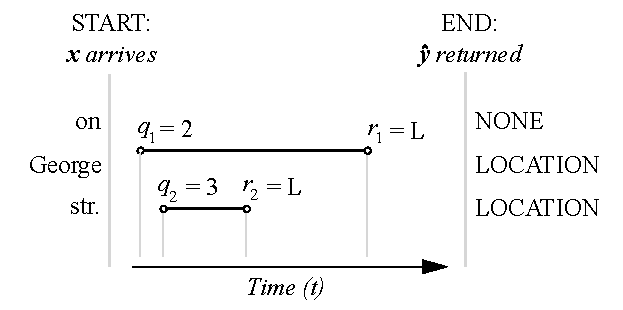
\includegraphics[width=\textwidth]{figures/piano-roll.pdf}
      \caption{Structured prediction behavior over time}
    \end{subfigure}
    \hfill
    \begin{subfigure}[b]{0.38\textwidth}
      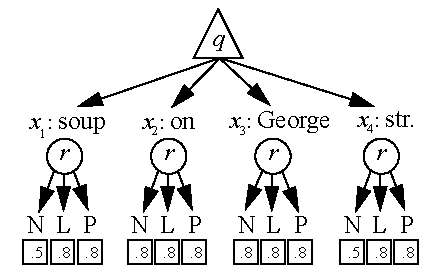
\includegraphics[width=\textwidth,height=0.23\textheight,keepaspectratio]{figures/single-move.pdf}\\[1.7ex]
      \caption{Single-query game tree}
    \end{subfigure}
  \end{centering}
\caption{Example behavior while running structure prediction on the tweet ``Soup on George str.''
We omit the \scres{} from the game tree for visual clarity.
}
\label{fig:game-tree}
\end{figure}


% ARUN: This is a little too much detail too early.  
% Define game top-down
% We define a stochastic game with two players, the system and the crowd.
% The system gets ``woken up'' every time something in the environment changes, and is allowed to make a move.
% The game starts with a $\bx$ arriving in need of a label, and the system must make a decision.
% Possible decisions are TURN\_IN, WAIT, and launching a query $q_0$ on one of the variables $\by_i$.
% If the system decides to TURN\_IN, the best guess $P_{\theta}(\bx|\by)$


% High-level what is the game?
We model on-the-job learning as a stochastic game with two players: the system and the crowd.
The game starts by the system receiving input $\bx$ and ends when the system turns in a set of labels $\by = (y_1, \ldots, y_n)$. 
During the system's turn, the system may choose an action $q \in \{1, \ldots, n\}$ to ask the crowd to label $y_q$. 
The system may also choose 
the wait action ($q = \acwait$) to wait for the crowd to respond to any pending queries
or
the return action ($q = \acret$) to terminate the game and return its best estimate given responses received so.\footnote{When $q = \acwait$ or $q = \acret$, $y_q$ is not defined and is ignored.}
When the wait action is chosen, the turn switches to the crowd, which provides a response $r$ to a pending query.
The key challenge is to determine which action the system should take during its turn.
For this, we appeal to Bayesian decision theory.

% How is the game played? maximizing utility under the model, which will be subsequently.
Under Bayesian decision theory, the \emph{optimal choice} of actions $\bq = (q_1, \ldots, q_k)$ for the system is the set of actions that attain the maximum expected utility (i.e.\ value) for the game:
\begin{align}
  \label{eqn:value}
V^* = \max_{\bq} \E_{p(\br \mid \bx, \bq)}[U(\bq, \br)],
\end{align}
where $\br = (r_1, \ldots, r_k)$ are the responses to the queries, $p(\br \mid \bx, \bq)$ is the system's model of the environment and $U(\bq, \br)$ is the utility which captures the cost of making the queries and the accuracy of the predictions given the responses. 
We will define these latter two quantities next.
%We will define these latter two quantities after looking at the example below:

%The \emph{value} of the game is the maximum expected utility:
%\begin{align}
%  V^* = \max_q \E_{p(r \mid \bx, q)}[U(q, r)],
%\end{align}
%and the \emph{optimal policy} is to choose the action $q$ that attains $V^*$.

% Arun: I don't think this is very useful -V
%Note that the system computes the $V^*$ by only \emph{simulating} possible futures, not by actually querying the crowd.

% Example time!
%Let us look at the example in \figureref{game-tree} more intuitively:
%querying one of the end positions ($q = 1$ or $q = 4$),
%is less informative than choosing the middle positions ($q = 2$ or $q = 3$),
%assuming the model propagates information between adjacent positions.
%Indeed, the expected utilities with a uniform distribution over $r$
%are $0.7$, $0.8$, $0.8$, and $0.7$, respectively, and so both $q = 2$ and $q = 3$ are optimal actions.

%Note that the system computes the $V^*$ by only \emph{simulating} possible futures, not actually querying the crowd.
%The simulation is based on the transition probabilities $p(r \mid \bx, q)$ and the utilities $U(q, r)$, which are based on a probabilistic model that connects input, output, responses, and time delays.

% Start model.
\paragraph{Environment model.}

We now define the model of the environment that the agent uses.
Given input $\bx$ and queries $\bq = (q_1, \dots, q_k)$ issued at times $\bs = (s_1, \dots, s_k)$,
we define a distribution over the output $\by$, responses $\br = (r_1, \dots, r_k)$
and response times $\bt = (t_1, \dots, t_k)$ as follows:
\begin{align}
  \label{eqn:dynamics}
%p(\by, \br, \bt \mid \bx, \bq) \eqdef \p(\by \given \bx) \prod_{i=1}^k \presp(r_i \mid \bx, \by, q_i) \ptime(t_i \mid \bx, \by, q_i, s_i).
p(\by, \br, \bt \mid \bx, \bq) \eqdef \p(\by \given \bx) \prod_{i=1}^k \presp(r_i \mid y_{q_i}) \ptime(t_i \mid s_i).
\end{align}
The three components, specified by the user, are as follows:
First, $\p(\by \given \bx)$ is the \emph{prediction model} (e.g.\ a standard linear-chain CRF).
Second, $\presp(r \given y_q)$ is the \emph{response model} which describes the distribution of the crowd's response $r$ for a given a query $q$ when the true answer is $y_q$.
%
If the crowd workers were infallible we could define $\presp(r \given y_q)$ to be $1$ iff $r = y_q$, but annotation errors are typical in practice. 
In our experiments, we model $\presp(r \given y_q)$ using an estimated confusion matrix.
%
Finally, $\ptime(t \given s)$ is the \emph{time delay model}, which governs how long a given query $q$ will take. While, in reality, $t$ depends on many factors including the input, in the interest of simplicity we assume $t - s$ to be drawn from a gamma distribution with globally fixed parameters.\footnote{
Of course, both $\presp$ and $\ptime$ can easily be extended to depend arbitrarily on the input $\bx$.}
We also define the \emph{response at time $\tau$}, $r[\tau]$, to be $r$ if $\tau > t$ and $\emptyset$ otherwise.

% Doing things with the model
Given this full model, we can compute $p(\br \mid \bx, \bq)$ simply by marginalizing out $\by$ and $\bt$ from \equationref{dynamics}.
We can also compute the distribution over responses at a particular time $\tau$, $p(\br[\tau] \given \bx, \bq)$, where $\br[\tau] = (r_1[\tau], \ldots, r_k[\tau])$.
% Describe the simplifications on how time is moved forward, with possibly an example

\paragraph{Utility.}

%The simulation dynamics model defines the transition probabilities of the game through various conditioning and marginalization operations.
We now define the utility of the game at time $\tau$, which must trade off two things.
The first is the accuracy of the MAP estimate according to the model's best guess of $\by$ incorporating all responses received by time $\tau$.
The second is the cost of making queries: a (monetary) cost $\weightmoney$ per query made and penalty of $\weighttime$ per unit of time taken.
Formally, the utility is defined as follows:
\begin{align}
  \label{eqn:utility}
  U_\tau(\bq, \bs, \br, \bt) &\eqdef F(p(\by \given \bx, \bq, \bs, \br[\tau], \bt)) - (k \weightmoney + \tau \weighttime), \\
  F(q) &= \E_{q(\by)}[\accuracy(\arg\max_{\by'} q(\by'))].
\end{align}
%Importantly, we are only conditioning on the responses $\br[t]$ that are available at time $t$.

% Behavior!
\paragraph{Behavior.}
If we had already made one query $q_1$ and gotten a response $r_1$,
we can incorporate the evidence, which will propagate through the CRF
and inform the distribution over possible responses $r_2$ for the next query $q_2$:
$p(r_2 \mid \bx, q_1, r_1, q_2)$.

\todo{WEIRD}
The temporal aspect of the model also allows for interesting possibilities
and is important for handling asynchronous queries and responses.
Suppose we made a query $q_1$ at time $s_1$ but have not yet gotten response $r_1$.
We might still want to ask for various probabilities \emph{at time} $t$,
which involves integrating over possible future responses $r_1$ and response times $t_1$.
Formally, define $r_i[t]$ to be the response at time $t$, which is equal to $r_i$ if $t_i \le t$
or $\emptyset$ if $t_i > t$.
Then we could ask about the probability of a response $r_2$ at time $t$,
which integrates over the possibility of having received $r_1$ or not:
\begin{align}
p(r_2[t] \mid \bx, q_1, q_2) = p(t_1 \le t \mid s_1) p(r_2[t] \mid \bx, q_1, r_1, q_2) + p(t_1 > t \mid s_1) p(r_2[t] \mid \bx, q_2).
\end{align}

Let us revisit the example in \figureref{game-tree} by looking at the game tree on the right where the system turns in an answer after a single query.
The square leaf nodes store the value of obtaining responses for each query.
Intuitively, because the model (a linear-chain CRF) propagates information between adjacent labels, querying one of the end positions ($q = 1$ or $q = 4$) is less informative than the middle positions ($q = 2$ or $q = 3$).
Indeed, this is reflected in the expected utilities of each query: with a uniform distribution over the responses, they are $0.7$, $0.8$, $0.8$, and $0.7$ respectively. Thus, both $q = 2$ and $q = 3$ are optimal actions.
\todo{this is a bit of a lame example.}

\paragraph{Efficient Monte-Carlo inference.}
%\paragraph{Putting it together.}

% Talk more about how the game is played / simulated.
% Talk more about how the game is optimized.
\todo{Make simulation stuff an algorithm box.}

Having defined the simulation dynamics and utility, we can now define the full game tree,
which is an extension of our initial example in \figureref{game-tree}~(right).
The technical challenge here is to incorporate the modeling of continuous time
into a traditionally discrete game tree.
A naive approach might be to discretize time and treat each level of the game
tree as a time step, but this discretization is inefficient.
Our strategy is to consider only represent game states corresponding to pivotal times $t$
and model waiting times as random actions played by the crowd.
%\citep{guo2009continuous}

% Game state, abstract goal
More formally, a \emph{game state} $s = (\now, \bq, \bs, \br, \bt)$
consists of the current time $t$, the queries $\bq$ issued at time $\bs$,
responses $\br$ that have be received at time $\bt$.
We assume that all queries $q_1, \dots, q_{k-1}$ have been issued,
but the last query $q_k$ has yet to be;
and some subset of responses in $r_1, \dots, r_{k-1}$ have been received,
and the rest are ``in flight.''
We focus on the problem of deciding (i) what to query ($q_k$)
and (ii) when to query ($s_k$) to maximize expected utility
at some future $\deadline$ (see \figureref{game-tree}~(left) for reference).
Recall the intuition: if $\deadline$ is near, then we would want to query
many labels in parallel; otherwise, we should operate more sequentially,
so as to be more adaptive.

% Describe game tree
At each state $s$ in the game tree in which it is the system's turn,
we query a position $q_k \in \{1, \dots, n\}$ (not necessarily new)
or wait until ($q_k = \emptyset$);
the successor state simply incorporates $q_k$.
If it is the crowd's turn,
then we sample the time of the first ``in flight'' response along with its value.
Formally, let $F = \{ 1 \le j \le k-1 : q_j \neq \emptyset \wedge r_j = \emptyset \}$ be the ``in flight'' queries.
Sample $t_j$ according to the time delay model for each $j \in F$
and take the earliest event $j^* = \arg\min_{j \in F} t_j$;
the actual response $r_{j^*}$ is drawn independently from the dynamics model conditioned on the queries and responses
in the state $s$;
the successor state incorporates $r_{j^*}$ and $t_{j^*}$ and advances time from $\now$ to $t_{j^*}$.
Technically, the optimal strategy might be to wait for an intermediate amount of time before $t_{j^*}$,
so our restriction to considering decisions only at response times is an approximation.

The following example shows one path over the states of the game tree corresponding to \figureref{game-tree}~(left),
where the system takes action $q_2 = 4$ (labeling \nl{str.}) and then the crowd responds
at time $1.7$ with $r_2 = \scloc$.
Note that the response $r_1$ for $q_1 = 3$ (\nl{George}) is still pending.
\begin{center}
\begin{tabular}{|ll|}
  \hline $\now = 1$ & \\
  \hline
  $q_1 = 3$         & $q_2 = \emptyset$ \\
  $r_1 = \emptyset$ & $r_2 = \emptyset$ \\
  \hline
\end{tabular}
$\stackrel{\text{\small system}}{\implies}$
\begin{tabular}{|ll|}
  \hline $\now = 1$ & \\
  \hline
  $q_1 = 3$         & $q_2 = 4$ \\
  $r_1 = \emptyset$ & $r_2 = \emptyset$ \\
  \hline
\end{tabular}
$\stackrel{\text{\small crowd}}{\implies}$
\begin{tabular}{|ll|}
  \hline $\now = 1.7$ & \\
  \hline
  $q_1 = 3$         & $q_2 = 4$ \\
  $r_1 = \emptyset$ & $r_2 = \text{\scloc}$ \\
  \hline
\end{tabular}
\end{center}

%\paragraph{Prediction model.}
% PL: form isn't relevant here since later we use other types of models anyway
%Assume our model
%We consider the family of conditional random fields
%exponential models, a popular class of models that include logistic regression
%and conditional random fields.
%Let $\bx$ be a given input, then the labels $\by = y_1, \ldots, y_n \in \{1,
%\dots, L\}$ are generated by the following conditional distribution:
%\begin{align*}
%  \p(\by \given \bx) 
%  &\propto \exp(\theta^\top \phi(\bx, \by)),
%\end{align*}
%where $\phi(\bx, \by)$ are features
%and $\theta$ are model parameters.
%In this paper, $\p(\by \given \bx) We assume that inference is efficient, which it is
%for our chain-structured models.
%(e.g.\ $\phi$ factorizes over the
%labels $\by$) or otherwise admits efficient marginal computation.

%For example, the model in \figureref{crf} is a linear-chain conditional random
%field. The input is the sequence of words in the tweet and the output is a
%label in the set \scnone, \scres, \scloc{} and \scper. Marginal inference can
%be efficiently computed using the Viterbi algorithm.

%Conventionally, we are given a training dataset $\sD = \{\bx_i, \by_i\}$ and can learn $\theta$ by optimizing the convex log-likelihood objective $\sL(\theta) = \sum_{t=1}^T \log \p(\by\oft{t} \given \bx\oft{t})$.
%In our setting, however, we do not observe the gold labels $\by$. 
%Instead, we can ask the crowd to provide a ``measurement'' for some subset of the labels.
%Let $\Sigma = \{\sigma_i\}$ be the set of possible measurements we can ask the crowd for and 
%let $\by_\sigma \subseteq \by$ be the subset of labels queried.

%\paragraph{Response model.}
%Let $q \in \{1, \ldots, n\}$ be a query on for the label $y_q$.
%We model the response, $r$, with an exponential measurement model:
%\begin{align*}
%  p_\beta(r \given x, y, q) 
%  &\propto \exp \left( \beta^\top\psi(\bx, y_q, r) \right),
%\end{align*}
%where $\beta$ and $\psi$ are extra parameters and features for the human error model. 
%%The choice of an exponential model allows us to simply include measurements as an additional factor.
%\figureref{crf}(c) shows the original graph with additional measurement nodes.
%A simple human error model is to return the true label with probability $1-\epsilon$ and a random label otherwise.
%In our running example, some classes, e.g.\ $\textsc{none}$, are more easily identified than others: in this setting responses can be modeled to be sampled from a confusion matrix.
%
%Finally, we model delay to be drawn from a Gamma distribution: $\tau \sim \Gamma$\footnote{We assume here for simplicity that the response delays are independent of the input and which label is being queried. The model can easily be generalized to incorporate these settings.}.
%\ac{The gamma is missing parameters.}
%Note that the total time taken on a prediction, $t$, depends not only on how many requests are made, but also when they are scheduled.
%%We study the problem of how to best schedule multiple requests in \sectionref{async}.
%
%Next, we describe how we use our models to predict labels and learn from partial feedback.

%\paragraph{Making predictions.}
%Given parameters $\theta, \beta$ and responses $r_1, \ldots, r_m$, our model makes predictions using maximum likelihood:
%$\byt \given \bx, r_1, \ldots r_m = \argmax_{\by} \p(\by \given \bx, r_1, \ldots r_m)$.
%
%\paragraph{Learning from responses.}
%Recall that we do not have gold labels for our data, but only noisy measurements: we do not have supervised examples to learn from. 
%As a simple heuristic, we use the output from our model as gold labels and update our parameters $\theta$ periodically.  
%We consider the response parameters $\beta$ to be fixed a priori.
%The time delay parameters can easily be estimated from the observed response delays.
%%In future work, we plan to explore using (online) expectation-maximization to jointly learn parameters for our model and the human error model in an unsupervised fashion.
%
%\paragraph{Computing expected utility.}
%
%\ac{Text}
%We cast this problem in the Bayesian decision theoretic framework: our objective is to maximize our expected utility under our current model,
%$\p(\by \given \bx, \br)$:
%\begin{align*}
%  u &= \E_{\by \sim \p(\cdot \given \bx, \br)}[1 - \ell(\by, \byt) + C(\bq, t)].
%\end{align*}

